% citazioni dall bibliografia:
% \textsuperscript{\cite{cas}}
%
% codice con linguaggio + caption:
% \begin{lstlisting}[language=xml, caption=Richiesta per un Access Token]code\end{lstlisting}
%
% immagine + caption + label (utile per \ref{valore_label}
%\begin{figure}[H]
%\begin{center}
%    \includegraphics [width=4in]{federa_sequenza.eps}
%\caption{Diagramma di sequeza per Autenticazione Federata}
%\label{autenticazioneFederata}
%\end{center}
%\end{figure}

\documentclass{article}
\usepackage{graphicx}
\usepackage{epstopdf}
\usepackage{wrapfig}
\usepackage{color}
\usepackage[utf8x]{inputenc}
\usepackage[T1]{fontenc}
\usepackage{enumitem}
\usepackage{listings}
\usepackage{color}
\usepackage[a4paper]{geometry}
\usepackage{amsmath}
\usepackage{amssymb}
\usepackage{mathpazo,graphics,graphicx,amsopn,url, epsf}
% Include the helvet package (helvetica font)
\usepackage[scaled]{helvet}
\usepackage[toc,page]{appendix}
\usepackage{float}
\usepackage[font={scriptsize,it}]{caption}

% Set the default font to be sans-seriF
\renewcommand*{\familydefault}{\sfdefault}

% Change 'table of contents' -> contents -> to italian 'Indice'
\renewcommand{\contentsname}{Indice}

% Change the 'figure' caption to the italian 'figura'
\renewcommand{\figurename}{Figura}

% Add a caption to lstlisting (code)
\renewcommand{\lstlistingname}{Codice}

% Renename References to Bibliografia
\renewcommand{\refname}{Sitografia}

\definecolor{dkgreen}{rgb}{0,0.6,0}
\definecolor{mauve}{rgb}{0.58,0,0.82}
\definecolor{lightgray}{gray}{0.5}

\lstset{frame=tb,
    aboveskip=3mm,
    belowskip=3mm,
    showstringspaces=false,
    columns=flexible,
    basicstyle={\small\ttfamily},
    numbers=none,
    numberstyle=\tiny\color{lightgray},
    keywordstyle=\color{blue},
    commentstyle=\color{dkgreen},
    stringstyle=\color{mauve},
    breaklines=true,
    breakatwhitespace=true,
    captionpos=b,
    tabsize=2,
}

\lstset{literate=
    {á}{{\'a}}1 {é}{{\'e}}1 {í}{{\'i}}1 {ó}{{\'o}}1 {ú}{{\'u}}1
    {Á}{{\'A}}1 {É}{{\'E}}1 {Í}{{\'I}}1 {Ó}{{\'O}}1 {Ú}{{\'U}}1
    {à}{{\`a}}1 {è}{{\'e}}1 {ì}{{\`i}}1 {ò}{{\`o}}1 {ù}{{\`u}}1
    {À}{{\`A}}1 {È}{{\'E}}1 {Ì}{{\`I}}1 {Ò}{{\`O}}1 {Ù}{{\`U}}1
    {ä}{{\"a}}1 {ë}{{\"e}}1 {ï}{{\"i}}1 {ö}{{\"o}}1 {ü}{{\"u}}1
    {Ä}{{\"A}}1 {Ë}{{\"E}}1 {Ï}{{\"I}}1 {Ö}{{\"O}}1 {Ü}{{\"U}}1
    {â}{{\^a}}1 {ê}{{\^e}}1 {î}{{\^i}}1 {ô}{{\^o}}1 {û}{{\^u}}1
    {Â}{{\^A}}1 {Ê}{{\^E}}1 {Î}{{\^I}}1 {Ô}{{\^O}}1 {Û}{{\^U}}1
    {œ}{{\oe}}1 {Œ}{{\OE}}1 {æ}{{\ae}}1 {Æ}{{\AE}}1 {ß}{{\ss}}1
    {ç}{{\c c}}1 {Ç}{{\c C}}1 {ø}{{\o}}1 {å}{{\r a}}1 {Å}{{\r A}}1
    {€}{{\EUR}}1 {£}{{\pounds}}1
}

\sloppy
\setlength{\parindent}{0pt}
\setlist[itemize]{itemsep=1pt}

\begin{document}

\begin{titlepage}
    \begin{center}
        {{\large{\textsc{ALMA MATER STUDIORUM - UNIVERSITÀ DI BOLOGNA}}}}
        \rule[0.1cm]{14cm}{0.1mm}
        \rule[0.5cm]{14cm}{0.6mm}
        {\textsc { SCUOLA DI INGEGNERIA E ARCHITETTURA } }\\
        {\small{\textsc { Corso di laurea in ingegneria informatica}}}
    \end{center}
    \vspace*{\fill}
    \begin{center}
        {\Large\textbf{SRS\\[1\baselineskip]
        Social Recommender System}} \\
    \end{center}
    \vspace*{\fill}
    \par
    \noindent
    \begin{minipage}[t]{0.47\textwidth}
        {\large{Relazione di:}\\[1\baselineskip]
        {\bf Paolo Galeone}}
    \end{minipage}
    \hfill
%\begin{minipage}[t]{0.47\textwidth}\raggedleft
%    {\large{Relatore:}\\[1\baselineskip]
%    {\bf Prof. Paolo Ciaccia}}
%\end{minipage}
    \vspace{20mm}
    \begin{center}
        \rule[0.1cm]{14cm}{0.1mm}
        \rule[0.5cm]{14cm}{0.6mm}
        Anno Accademico 2014/2015\\
%    Sessione II
    \end{center}
\end{titlepage}
\clearpage
\tableofcontents
\clearpage

\section{Introduzione}

L'obiettivo del progetto è quello di progettare ed implementare un sistema di raccomandazione (Recommender System, o come spesso abbreviato nel testo RecSys) integrabile all'interno di un qualsiasi social network che fornisca determinate API.

Nella prima sezione vengono brevemente descritti i Recommender System, portando alcuni esempi di casi d'uso in cui i RecSys hanno grande rilevanza.

Viene in seguito introdotta una classificazione basata sulla tipologia di filtering adottata (Content Based o Collaborative) e vengono introdotti i due task principali dei RecSys (i quali permettono una classificazione ancora più specifica): la item prediction e la Top-N reccomendation.

Nella sezione successiva si entra nel vivo del progetto di SRS (acronimo di Social Recommender System), il cui task è quello della Top-N reccomendation, utilizzando tecniche di Content Based Filtering (CBF).

Viene illustrata l'idea che ha portato alla sua creazione, ponendo l'attenzione sulle funzionalità elementari che ogni social network fornisce all'utente.

Nei capitoli successivi si passa alla fase di progettazione, la quale è supportata da una forte componente matematica a giustificazione delle scelte progettuali fatte.

In particolare si pone l'attenzione sull'insieme delle coppie (utente, argomento), e sulle varie frequenze delle azioni elementari (compiute dall'utente) che permettono di mettere in relazione la coppia (utente, argomento) e degli istanti temporali.

Infine si estraggono dei parametri in grado di identificare univocamente un utente all'interno di un piano associato ad un argomento. Rendendo così possibile il poter realizzare misure della distanza tra punti (utenti) e stimare quindi la similarità tra questi.

Nella parte finale viene mostrata l'architettura dell'implementazione di SRS, motivando il perché delle scelte progettuali fatte.

In fine, viene valutata la bontà della raccomandazione, utilizzando (tra gli altri) gli indicatori più comuni per la valutazione del task di Top-N reccomendation: precision e recall.
\clearpage
\section{Recommender System}
I recommender system (sistemi di raccomandazione) sono una sottoclasse degli information filtering system (sistemi di filtraggio delle informazioni) che cercano di predire la "valutazione" o la "preferenza" che un utente darebbe ad un elemento.

I recommender system sono un elemento chiave di molti servizi. Si pensi ad esempio ad Amazon\footnote{https://www.amazon.com/} il quale suggerisce prodotti correlati a quello appena
acquistato, in modo tale da spingere l'utente a valutarne la possibilità di acquisto ed incrementare così il suo fatturato.

Oppure a social network come Twitter\footnote{https://www.twitter.com}, il quale basa tutta la creazione della rete sociale dell'utente in base ai suggerimenti basati sugli interessi che è in grado di inferire dal comportamento dell'utente.

Esistono alcune metodologie di filtering fondamentali, che permettono di classificare i RecSys in base al loro modo di trattare (filtrare) i dati.

\subsection{Metodologie di filtering fondamentali}
\begin{enumerate}
    \item \textbf{Collaborative filtering (CF)}: cercano di dare suggerimenti in base al comportamento di utenti simili oppure che hanno eseguito stesse azioni.

        Questo tipo di RecSys necessita quindi di avere informazioni sul comportamento degli utenti, in modo tale da poterli classificare e sfruttare queste informazioni per generare i suggerimenti.

        Ad esempio in un e-commerce, il RecSys usando tecniche di CF può suggerire prodotti "collegati" in qualche modo a quello appena acquistato, mostrando ad esempio cosa altri utenti che hanno acquistato lo stesso prodotto hanno aggiunto nel carrello nello stesso acquisto.

    \item \textbf{Content based filtering (CBF)}: cercano di dare suggerimenti all'utente in base alle caratteristiche degli elementi ai quali si dimostra interessato.

        Ad esempio in un e-commerce, il RecSys usando tecniche di CBF può suggerire prodotti simili a quello appena acquistato/visualizzato in modo tale da spingere l'utente a valutare le alternative.
    \item \textbf{Hybrid Recommender System}: usano sia tecniche di CF che di CBF
\end{enumerate}
Moltre alte metodologie di filtering esistono e molte altre ne stanno nascendo in quanto il campo dei RecSys è in rapidissima espansione.
\clearpage
\section{SRS}
L'idea alla base di SRS è quella di realizzare un sistema di raccomandazione in grado di suggerire una lista di N utenti "simili" all'utente al quale sono dirette le raccomandazioni.

Questo tipo di raccomandazione è detta \textbf{Top-N recommendation}.

La Top-N recommendation è una variante di (o una modalità di valutazione per) il task di \textbf{item prediction}.

Il compito specifico è quello di predire i migliori N elementi, cioè gli elementi che più di tutti soddisfano i criteri di valutazione (che siano i più simili o comunque quelli che seguono la metrica scelta).


Solo questi elementi saranno mostrati all'utente o presi in considerazione per la valutazione dei risultati.

L'Item prediction (o item recommendation) è il task che consiste nel predire elementi che potrebbero piacere ad un utente, basato sul comportamento dell'utente (e possibilmente altre informazioni).

La Top-N recommendation è un task in contrapposizione con un altro task fondamentale dei RecSys, cioè la \textbf{Rating Prediction}.

La Rating Prediction ha come obiettivo quello di predire la valutazione che un'utente darà ad un determinato elemento in base alle valutazioni passate (usando CF) o altre informazioni.

Per poter offrire raccomandazioni di qualità è necessario analizzare dettagliatamente le informazioni che il social ci può fornire, così da poter suggerire all'utente utenti simili a lui.

Estrarre i dati e metterli in relazione tra di loro è il compito più delicato delle fase di progettazione di un RecSys, come è ovvio, se si lavora su informazioni poco rilevanti i suggerimenti saranno poco rilevanti (e quindi inutili per l'utente finale).

SRS ha come obiettivo quello si suggerire utenti simili, nel seguito sarà considerata la seguente assunzione:

\begin{quotation}
    \noindent{Due utenti sono simili quando parlano di frequente di argomenti comuni.}
\end{quotation}

\subsection{L'idea}
Anche il mondo dei social network, come quello dei RecSys, è in rapidissima crescita.

Analizzando i più comuni social network (ed anche alcuni di quelli di nicchia) è facile notare che ognuno di questi offre funzionalità comuni a tutti, che chiameremo nel seguito Funzionalità elementari.
\subsection{Funzionalità elementari} \label{ss:fe}
Le funzionalità elementari identificate sono:
\begin{enumerate}
    \item Inserire \#hashtag\footnote{Gli hashtag sono un tipo di tag usato dai social network per permettere agli utenti di etichettare (quindi classificare) il contenuto. La lo struttura è nella forma \# (hash) + tag, dove tag è la categoria in cui l'utente vuole inserire il messaggio.} per classificare il contenuto
    \item Inserire commenti
    \item Esprimere un parere sotto forma di votazione/valutazione
    \item Ricercare per argomento: solitamente premendo sull' \#hashtag
\end{enumerate}

Dato che ogni social network offre queste funzionalità:
\begin{quotation}
    \noindent{perché non sfruttare queste funzionalità per creare un sistema di raccomandazione utenti generico?}
\end{quotation}

Cioè un RecSys valido per ogni social network che esponga API per ottenere le informazioni necessarie o installi SRS localmente, facendolo interagire con il database.

Nel seguito si mostrerà l'implementazione per il social network NERDZ\footnote{https://www.nerdz.eu/: una sintetica descrizione del social network si può trovare in appendice B} del quale sono l'ideatore e sviluppatore.

\subsection{Estrazione dei dati}
Le funzionalità elementari ({\ref{ss:fe}) ci offrono la possibilità di estrarre relazioni tra utenti ed argomenti e di conseguenza tra utenti ed utenti.

L'idea alla base di SRS è quella di sfruttare le coppie $(\text{utente}, \text{argomento})$.

Per offrire una raccomandazione il più possibile corretta si cerca ogni possibile relazione dell'utente con l'argomento. In particolare la ricerca è effettuata tra: 
\begin{enumerate}
    \item i post che l'utente ha volontariamente classificato tramite gli \#hashtag
    \item i post classificati (da qualcuno, non necessariamente dall'utente in esame) in cui l'utente ha commentato
    \item i post classificati per i quali l'utente ha espresso una valutazione positiva/negativa
    \item i commenti ai post classificati per i quali l'utente ha espresso una valutazione positiva/negativa
    \item le ricerche dell'utente di determinati argomenti (cioè quelle partite digitando volontariamente un \#hashtag oppure partite perché l'utente ha cliccato su un \#hashtag di interesse)
\end{enumerate}

Inoltre è fondamentale tenere conto dell'\textbf{istante temporale} nel quale l'utente ha creato il collegamento con l'argomento, in quanto le abitudini degli utenti cambiano nel tempo.

Formalmente stiamo costruendo due insiemi:
\begin{enumerate}
    \item L'insieme di tutte le coppie $(\text{utente}, \text{argomento})$
        $$ UT = \left\{ (U, T) : \text{U is in some relation with T}, U \in Users \land T \in Topics \right\} $$
    \item L'insieme di tutte le coppie $(\text{utente}, \text{argomento})$ nell'intervallo $R$:
        $$ UT_R = \left\{ (U, T) : \text{U is in some relation with T}, U \in Users \land T \in Topics \land R = Time Range \right\}$$
\end{enumerate}

Quindi si ha:
$$ UT = \bigcup_{R \in ]-\infty, Now]} UT_R $$
Per intervalli $R$ disgiunti.

\clearpage
\subsection{Attribuzione di un valore numerico alla coppia $(\text{utente}, \text{argomento})$}
All'interno dell'intervallo temporale considerato, l'utente potrebbe quindi aver eseguito più azioni elementari, che la sola estrazione delle coppie (utente, argomento) non considera.

A partire dalle coppie $(\text{utente}, \text{argomento})$ si può calcolare \textbf{la frequenza delle azioni elementari nell'intervallo}: così da poter ottenere un valore numerico che sia un buon indicatore da associare alla coppia considerata.

La frequenza all'interno dell'intervallo è un buon indicatore in quanto esprime quanto spesso l'utente parla di un argomento.

Ovviamente più un utente parla di un argomento, più l'argomento gli interessa (oppure lo critica, ma anche la critica è la manifestazione di un interesse).

Quindi costruiamo l'insieme:

$$ UTA_f(u,t,r) = \left\{ \begin{cases}\begin{aligned} \frac {|\left\{t \in Topics, r = R, u \in Users, action = i\right\}|} {|A = \left\{r=R, u \in Users, action=i\right\}|} \in [0,1], |A| > 0\\ 0, |A| = 0 \end{aligned} \end{cases} : i = \text{elementary action} \right\} $$

User Topic Action Frequency ($UTA_f$) è l'insieme delle frequenze delle azioni elementari associate all'utente $u$, per il topic $t$ nell'intervallo di tempo $r$ fissato.

Notare che la frequenza definita ha sempre un valore $\in [0,1]$ e che è considerata nulla quando l'utente non ha parlato di questo argomento.

Chiamiamo $SRS\_DB$, l'unione di tutti gli $UTA_f$, con $r$ variabile.

$$ SRS\_DB = \bigcup\limits_{u \in Users, t \in Topics, r \in ]-\infty, Now]}{UTA_f(u,t,r)} $$

\subsection{Influenza del tempo nella raccomandazione}
A questo punto abbiamo l'insieme $SRS\_DB$ contenente gli insiemi delle frequenze delle azioni elementari per ogni coppia $(\text{utente}, \text{argomento})$ durante ogni intervallo di tempo $R$ prestabilito, ipoteticamente da un tempo $-\infty$ all'istante attuale. 

Nella pratica:
\begin{enumerate}
    \item l'istante iniziale è il momento in cui è stato creato il primo contenuto classificato all'interno del social network
    \item l'intervallo di tempo $R$ è fissato ad un'ora (in prospettiva di un'esecuzione oraria del calcolo delle frequenze, in modo tale da avere dati omogenei nel tempo).
\end{enumerate}

Naturalmente le raccomandazioni che SRS dovrà dare non dovranno essere sola funzione degli argomenti comuni, ma anche essere in funzione del tempo.


Difatti è impensabile suggerire un'utente che era interessato ad \#argomento 2 anni fa (e poi il suo interesse è diminuito nel tempo fino ad esaurirsi) ad un utente che è interessato ad \#argomento ora. 

Quindi è necessario definire una funzione in grado di mettere in relazione le frequenze calcolate nei vari intervalli temporali, che esprima il grado di interesse dell'utente per l'argomento in funzione decrescente del tempo.

Questa funzione esprime \textbf{il peso associato alla coppia $(\text{utente}, \text{argomento})$}.

\subsubsection{Scelta della funzione peso}
Una delle funzioni più note il cui andamento è decrescente in funzione del tempo è l'\textbf{esponenziale negativo}: $$ Me^{-t} $$.

Una seconda funzione un po' più complessa, da me definita, è la \textbf{funzione gradino ricorsivamente definita}.

Il cui decremento (l'"altezza" del singolo scalino) è variabile in funzione del valore del parametro $\alpha$.

$$ B(t) = \begin{cases} \begin{aligned} M , t = t_0 \\ \frac{B(t + 1)}{\alpha}, t < t_0 \land 2 \leq \alpha <M \end{aligned} \end{cases} $$

In entrambe le funzioni si considera la variabile temporale \textbf{discreta} in quanto le rilevazioni temporali sono effettuate ad intervalli temporali di ampiezza $R$ (discreti).


La scelta è ricaduta sulla seconda funzione, in quanto maggiormente manipolabile variando il parametro $\alpha$.
Inoltre si dimostra (la dimostrazione è riportata in appendice A) che per valori di $\alpha < e$, $B(t)$ decresce più lentamente dell'esponenziale.

Inoltre $B(t)$ offre le \textbf{condizioni di stabilità} all'interno degli intervalli che desideriamo, in quanto è ragionevole pensare che gli interessi di un'utente siano stabili in determinati intervalli temporali.

Per SRS stiamo cercando una funzione che abbia valori "alti" (cioè prossimi o uguali ad $M$) per valori del tempo prossimi allo zero (cioè vicini all'istante attuale) e che siano stabili il più possibile per ogni intervallo di tempo unitario su cui questa è definita (in modo tale da poter offrire raccomandazioni il più possibile stabili con l'aumentare del numero di argomenti trattati).

Poi nel variare del tempo, è necessario che la funzione decresca rapidamente: in quanto le attività fatte in un tempo passato devono influenzare la raccomandazione in maniera minore di quelle attuali.

\begin{figure}[H]
    \begin{center}
        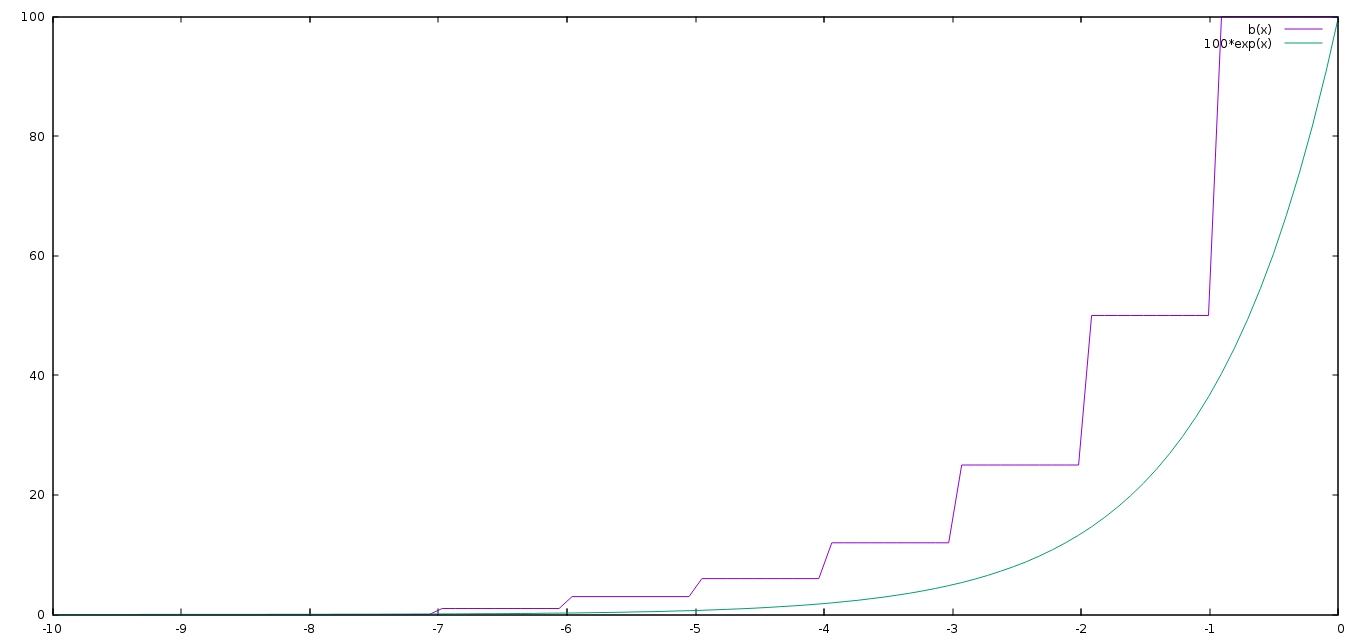
\includegraphics [width=5in]{images/confronto_b_e.eps}
        \caption{Confronto tra le funzioni B(t) ed e(t)}
        \label{fig:confronto_b_e}
    \end{center}
\end{figure}

In figura \ref{fig:confronto_b_e} viene mostrato un confronto tra le due funzioni, in cui è stato posto $M = 100$ e $\alpha = 2 < e$, in cui è evidente come $B(t)$ descresca più lentamente del'esponenziale negativo ed offra le condizioni di stabilità all'interno di intervalli discreti che cerchiamo.

Avendo trovato la funzione con l'andamento desiderato in funzione del tempo e con le determinate caratteristiche di stabilità, è necessario mettere in realzione le frequenze contenute nell'insieme $SRS\_DB$ con il tempo, definiamo quindi ora una funzione in grado di mettere in relazione queste due misure.

\subsubsection{Relazione frequenze peso}
L'insieme $SRS\_DB$ contiene le frequenze delle azioni elementari, eseguite dall'utente relativamente all'argomento, calcolate in intervalli temporali R.

Possiamo mettere in relazione quindi la funzione peso (temporale) con le frequenze calcolate, sfruttando l'intervallo di calcolo delle frequenze.

Decidendo di mantenere la dimensione del peso (cioè avere una dimensione $\in [0,M]$) e modularla in funzione delle frequenze, definisco:

$$ fw(u,T,R) = \begin{cases}\begin{aligned} 0, |\{u : \forall x( u \in Users \land (u,x)_{time} \in R)\}| = 0 \\ B(max\{t \in R\})^{ \frac{ \sum\limits_{u \in Users, T \in Topics, (u,T)_{time} \in R, i \leq n)}^{n}{f_i} } {n |\{u : \forall x( u \in Users \land (u,x)_{time} \in R)\}|} \in [0,1]} \in [0,M], \text{otherwise} \end{aligned} \end{cases} $$

La funzione $fw$ (frequency-weight) esprime questa relazione.


I parametri di ingresso sono: un utente $u$, un argomento $T$ ed un intervallo temporale $R$.

Calcolando questa funzione per ogni coppia $(\text{utente}, \text{argomento})$ all'interno di un intervallo $R$ otteniamo un valore $\in [0,M]$ in funzione \textbf{sia del tempo che della frequenza di relazione utente-argomento}.

Calcolando questo valore per $R = 28$ giorni (nel passato, a partire da oggi.\footnote{Ricordando inoltre che all'interno di $SRS\_DB$ abbiamo le frequenze orarie}) e sommando i risultati ottenuti, otteniamo un valore che mette in relazione la frequenza di relazione con l'argomento durante "un mese".


Ripetendo il procedimento per 12 intervalli ognuno distante dal successivo di -28 giorni, otteniamo una serie di valori che identifica la relazione durante l'anno.

$$ fw(u,T, 1y) = \sum\limits_{i=1}^{12}{fw(u,T, \text{Now} - 28\cdot i)} \leq M\sum\limits_{i=1}^{12}{\frac{1}{\alpha^i}} $$

La scelta di considerare come intervallo massimo 1 anno è del tutto arbitraria.

La funzione $B(t)$ evidentemente rende trascurabili i valori più distanti dall'istante iniziale, ma il suo comportamento è del tutto personalizzabile variando i parametri $M$ ed $\alpha$ (ovviamente aumentando $M$ e riducendo $\alpha$).

Inoltre abbiamo un'altra informazione che non è stata ancora utilizzata, che è il \textbf{numero di occorrenze della frequenza di relazione durante l'anno}.

$$ o(u,T,1y) = |\{u : u \in Users \land (u,T)_{time} \in ]Now-1y,Now]\}| $$

Cioè il numero di volte in cui l'utente ha creato un collegamento con l'argomento durante l'anno (all'interno delle rilevazioni fatte ad intervalli di ampiezza $R$).

Se si considera il totale delle relazioni utente, argomento (per ogni argomento) durante l'anno, otteniamo un insieme con cardinalità $o(u, 1y) >= o(u,T,1y)$

$$ o(u, 1y) = |\{u : \forall x(u \in Users \land (u,x)_{time} \in ]Now-1y, Now]\}|$$

Il rapporto tra le due grandezze ci da un valore $\in [0,1]$ che è la frequenza di relazione durante l'anno.

$$ \frac{o(u,T,1y)}{o(u,1y)} $$

Per ottenere una coppia di valori sulla stessa scala, possiamo normalizzare il valore ottenuto in $fw(u, T, 1y)$, dividendolo per l'estremo superiore dell'insieme dei valori che la somma delle serie può ottenere. Cioè:

$$ \frac{fw(u,T, 1y)}{M\sum\limits_{i=1}^{12}{\frac{1}{\alpha^i}}} \in [0,1]$$

A questo punto abbiamo \textbf{due coordinate nello spazio identificato dall'argomento} che ci permettono di identificare univocamente l'utente.
$$ \left|\left(\frac{fw(u,T, 1y)}{M\sum\limits_{i=1}^{12}{\frac{1}{\alpha^i}}}, \frac{o(u,T,1y)}{o(u,1y)} \right)\right| \in [0,1]$$

\subsection{Identificazione dell'utente negli spazi}
Riassumiamo i passi compiuti fino ad ora, mostrando l'annessa rappresentazione geometrica.

\begin{enumerate}
    \item Partendo da un piano, contenente sull'asse $x$ gli utenti e sull'asse $y$ gli argomenti, abbiamo estratto le coppie $(\text{utente}, \text{argomento})$ (cioè abbiamo valutato il valore della funzione $x = k$).
    \item Questa operazione di valutazione, ci ha permesso di isolare un insieme di valori, cioè tutti gli argomenti trattati dall'utente
    \item Per ogni coppia isolata, abbiamo calcolato la frequenza delle azioni elementari associata
    \item Abbiamo definito una funzione con un andamento particolare in funzione del tempo ad abbiamo creato la relazione tra la coppia ed il tempo, ottenendo così un valore, che abbiamo successivamente normalizzato per cadere nell'intervallo [0,1]
    \item Abbiamo normalizzato anche il valore della frequenza di relazione annuale, ottenendo così una coppia di valori, che per ogni piano che un argomento identifica, ci permette di individuare l'utente.
\end{enumerate}

A questo punto abbiamo un insieme di piani (identificati dagli argomenti), ognuno dei quali contiene un insieme di punti che sono gli utenti.

Si può quindi trovare \textbf{la distanza tra due utenti} semplicemente utilizzando la \textbf{distanza euclidea}.

Ricercando l'utente a distanza minore da quello in esame, all'interno di ogni piano in cui l'utente è presente, possiamo individuare gli utenti più affini con quello ricercato.
\clearpage
\subsection{Ordine della raccomandazione}

Ricordiamo che SRS ha come task quello di offrire una Top-N reccomendation, quindi l'ordine in cui le raccomandazioni verranno fornite è importante.

Si vuole raccomandare per prima utenti che siano il più affini possibili con l'utente in esame, e per ultimi quelli meno affini (ma comunque con una qualche affinità).

Per dare un ordine alla raccomandazione, possiamo sfruttare le distanze ottenute tra tutti gli utenti ed il numero di volte in cui gli utenti compaiono all'interno di un piano comune.

È evidente che se due utenti appaiono molto spesso, a distanze ravvicinate, su piani comuni, questi due utenti saranno molto simili.

Per ottenere quindi un ordine di raccomandazione creiamo una relazione tra questi due valori, semplicemente usando la \textbf{media aritmetica}.

Gli utenti che in media sono più vicini a quello in esame, saranno i primi ad essere raccomandati.

\clearpage
\subsection{Implementazione}
\begin{wrapfigure}{r}{0.5\textwidth}
    \vspace{-20pt}
    \begin{center}
        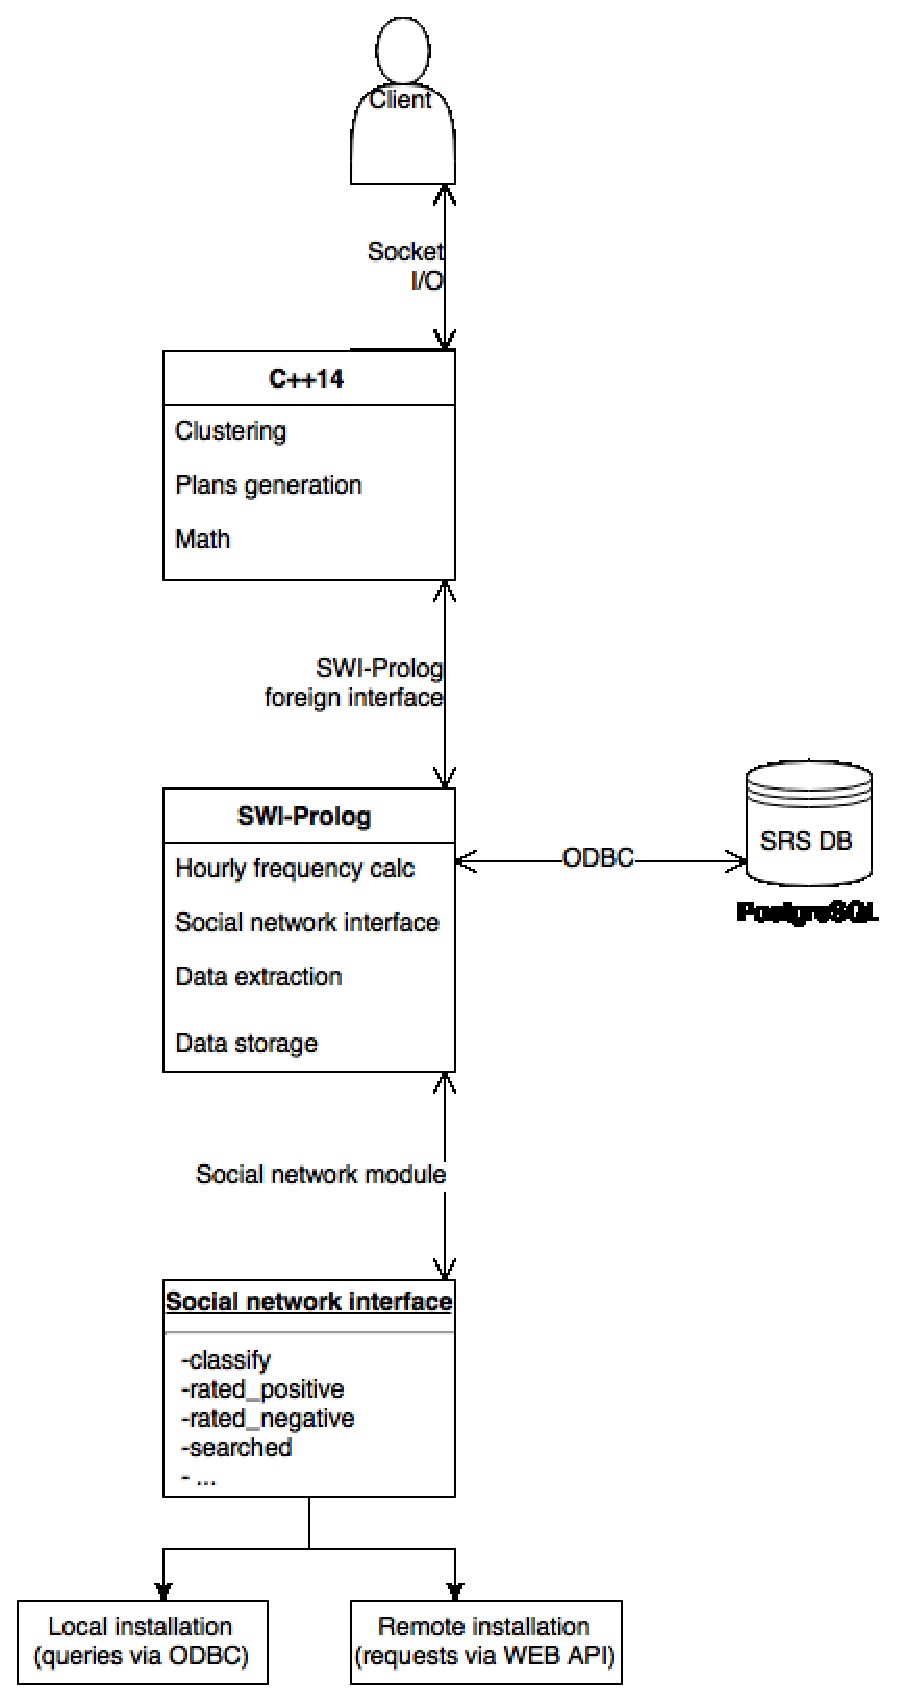
\includegraphics[width=0.48\textwidth]{images/arch.eps}
        \label{fig:arch}
    \end{center}
    \caption{Architettura di SRS}
    \vspace{-20pt}
\end{wrapfigure}

SRS è stato realizzato per essere il più generico possibile, utilizzando principalmente due strumenti molto diversi tra di loro ma con un puntoin comune che permette di potergli fare scambiare informazioni.

I due strumenti (linguaggi di programmazione) usati sono: Prolog (in particolare l'implementazione SWI-Prolog) e C++.

Come si può vedere della figura accanto, la parte che interagisce con il social network è stata realizzata in Prolog, la stessa parte si occupa anche di generare e memorizzare l'$SRS\_DB$ all'interno del database PostgreSQL\footnote{https://www.postgresql.org}.

SWI-Prolog mette a disposizione una \textit{foreign language interface}, cioè una maniera per poter permettere all'interprete prolog di essere inserito all'interno di altri software scritti in altri linguaggi ed interoperare con essi.

Sfruttando questa sua funzionalità, è stato possibile mettere in comunicazione il software scritto in C++, incaricato di eseguire i calcoli più pesanti (normalizzazioni, estrazione degli utenti dai piani, ricerche ottimizzate su strutture dati che Proog non fornisce, ecc) ed esporre il front-end con l'utente finale (che sarà il social network stesso).

\subsubsection{Prolog}
Prolog è stato scelto principalmente per la sua capacità di esprimere concetti complessi in Logica del Primo ordine e lavorare su questi in maniera molto semplice.

È stato così possibile effettuare un mapping tra le relazioni presenti nel database del social network ed entità logiche e lavorare in seguto su queste.

Per poter effettuare il mapping è stato utilizzato il modulo offerto da SWI-Prolog ODBC (Open DB Connectivity), il quale permette di interfacciarsi con dei database.

SRS utilizza ODBC sia per creare ed interrogare il suo database ($SRS\_DB$), che per interrogare il database del social network nel caso in cui SRS venga installato localmente (per ora unica implementazione disponibile per NERDZ).
\clearpage
La parte in prolog è stata realizzata in 3 moduli:
\begin{enumerate}
    \item l'interfaccia verso il social (nel caso di nerdz una lunga lista di query al database del social, fatte per ottenere i dati di interesse).
    \item il motore (engine.pl), il quale effettua i calcoli delle frequenze sui dati che l'interfaccia gli fornisce
    \item srs.pl, una semplice lista di predicati creati per essere utiliizzati dall'esterno (tramite la foreign interface). Interrogano $SRS\_DB$ e forniscono tutte le soluzioni all'interrogazione.
\end{enumerate}

\subsubsection{C++}
La scelta del C++ è stata dettata da due fattori:
\begin{enumerate}
    \item SWI-Prolog offre la foreign interface in C ed una (wrapper di quella in C), in C++, esponendo oggetti e semplificando quindi la fase di scrittura del codice.
    \item Il C++, nel suo standard più recente (C++14) offre nuove funzionalità (uso di lambda come funzioni di callback, una libreria standard più ricca, un sistema di tipi automatici\dots) che permettono di scrivere software in maniera migliore. Inoltre, visto l'intensivo uso di strutture dati complesse, quali vettori a grandezza dinamica e mappe (che rappresentano i vari piani) e la necessità di effettuare ricerche su questi elementi era necessario un linguaggio con buone performance in grando di eseguire calcoli in maniera molto rapide. La scelta del C++ è stata la più naturale.
\end{enumerate}

La parte realizzata in C++ è quella che esegue i calcoli più complessi e che espone l'interfaccia verso l'utente.

L'interazione con il client è stata realizzata tramte socket, cioè SRS sarà quindi un server, a cui il social farà richieste per ottenere le raccomandazioni.

Inoltre, vista la necessità di eseguire ogni ora l'aggiornamento delle frequenze, è facile scrivere uno script (da fare eseguire ogni ora) che vada ad istruire, tramite scrittura sul socket in ascolto, SRS per eseguire le operazioni richieste.

Scrivendo in questa maniera il software i vantaggi sono evidenti.

Uno tra tutti è quello della generazione dei piani una sola volta durante un intervallo temporale, con successivo salvataggio di questi in RAM.

In questo modo ogni richiesta di raccomandazione utilizzerà i piani generati senza doverli generare ad ogni esecuzione (cosa necessaria invece se lo sviluppo fosse stato fatto come eseguibile non server).

La realizzazione è stata fatta sfruttando appieno il paradigma di programmazione ad oggetti (quindi sono stati creati oggetti, ognuno dei quali rappresenta un'entità del "mondo reale" da noi descritto).

\clearpage
\subsection{Valutazione della raccomandazione}
\begin{quotation}
    \noindent{
        Due classi di metriche possono essere usate per valutare gli algoritmi di raccomandazione: le metriche d'errore e le metriche di classificaizone.

        Le metriche d'errore valutano l'errore tra $r_{ij}$, la valutazione attualmente data dall'utente $i$ all'elemento $j$, e $\bar{r_{ij}}$, il valore predetto dall'algoritmo di raccomandazione.

        Una delle metriche d'errore maggiormente utilizzata è la RMSE (Root Mean Squadred Error).

        Nonostante sia molto utilizzata per valutare i vari RecSys, le metriche d'errore non hanno significato per il task di raccomandazione Top-N, in quanto ci troviamo in un contesto nel quale non siamo interessati nel predire la valutazione di un elemento con precisione, ma piuttosto siamo interessati nel fornire all'utente una lista ordinata di N elementi che potrebbero interessargli.

        Per misurare precisamente l'accuratezza della raccomandazione, necessitiamo d'utilizzare metriche di \textit{interofmation-retrieval}, le quali sono in grado di misurare la probabilità che il RecSys dia un suggerimento corretto o meno all'utente.

        Quando si usano metriche di classificazione, dobbiamo distunguere tra 4 tipi di raccomandazione:
        \begin{enumerate}
            \item True Positive (TP): se il sistema suggerisce un elemento che effettivamente interessa all'utente.
            \item True Negative (TP): se il sistema non suggerisce un elemento che non interessa all'utente.
            \item False Positive (FP): se il sistema suggerisce un elemento all'utente che però non è di interesse
            \item False Negative (FN): se il sistema non suggerisce un elemento che è di interesse per l'utente
        \end{enumerate}

        Le più più popolari metriche di classificazione dell'accuratezza sono: \textbf{recall (sensitivity)} e \textbf{precision}.
        \begin{enumerate}
            \item $ TPR = \frac{TP}{TP + FN}$
            \item $ PPV = \frac{TP}{TP + FN}$
        \end{enumerate}
    }
\end{quotation}\textsuperscript{\cite{contentwise_tv}}

Come è evidente, il valore di Recall e Precision essendo funzione del campione sul quale vengono effettuate le misurazioni sono un buon indicatore solo se il campione è buono.

\subsubsection{Test}
Il campione usato per il test dell'accuratezza di SRS è un sottoinsieme degli utenti di NERDZ, i quali hanno un numero di followers e following non eccessivamente alto (cioè seguono solo una cerchia ristretta di utenti e non qualunque utente iscritto).

Così facendo possiamo ottenere valori di precision e recall significativi.

Il dataset di fatti reali è composto dalle coppie (A, B), in cui A segue l'utente B.

Il dataset di test è composto invece dalle raccomandazioni (o meglio, dall'affinità tra utenti che SRS calcola, includendo quindi anche nella raccomandazione gli utenti che già si seguono).

Viene creata così per ogni utente nel dataset di test la \textbf{matrice di confusione}, che riporta i 4 valori di TP, TP, FP e FN.

Per ogni utente calcoliamo così i valori di precision e recall (ed altre metriche, come mostrato sotto) e di questi valori ne calcoliamo la media per ottenere i valori generali.
\begin{lstlisting}[language=xml, caption=Alcuni risultati dai test sul dataset]
[+]     Testing for user 1898
[+] Building confusion matrixx...
Actual class:                   Followed    Not followed
Predicted class Followed        16          93
                Not followed    2           1829
Sensivity: 0.888889
False negative rate: 0.111111
Specificity: 0.951613
Fall out: 0.0483871
Precision: 0.146789
False discovery rate: 0.853211
Negative predictive value: 0.998908
F1 score: 0.251969

[+]     Testing for user 352
[+] Building confusion matrix...
Actual class:                   Followed    Not followed
Predicted class Followed        14          49
                Not followed    7           1870
Sensivity: 0.666667
False negative rate: 0.333333
Specificity: 0.974466
Fall out: 0.0255342
Precision: 0.222222
False discovery rate: 0.777778
Negative predictive value: 0.996271
F1 score: 0.333333
\end{lstlisting}

La media ottenuta (tra quelli mostrati e gli altri non mostrate per brevità) è:

\begin{lstlisting}[language=xml, caption=Alcuni risultati dai test sul dataset]
Sensivity: 0.514469
False negative rate: 0.485531
Specificity: 0.972019
Fall out: 0.0279813
Precision: 0.33543
False discovery rate: 0.66457
Negative predictive value: 0.986473
F1 score: 0.406091
\end{lstlisting}

Da notare che essendo SRS un recommender system che servirà per fare user linking (cioè creare collegamenti tra utenti, tramite follow), il valore della sensitività è destinato a variare in funzione che questi accettino o rifiutino la valutazione (inizino o meno a seguire l'utente).

\clearpage
\section{Conclusione e sviluppi futuri}
SRS è attualmente in grado di raccomandare utenti in base alla loro somiglianza in termini di relazione ad argomenti comuni.

Le prospettive per lo sviluppo di SRS sono molte.

Si potrebbero aggiungere tecniche di Collaborative Filtering in modo tale da offrire valutazioni non solo basate sulle coppie (utente, argomento) ma anche sulla somiglianza tra le abitudini dell'utente.

Si potrebbe far sì che a seguito dall'accetazione (o del rifiuto) del consiglio, SRS adegui le sue raccomandazioni future variando i suoi parametri di ordinamento per la Top-N reccomendation.

Il campo dei RecSys è in rapidissima evoluzione, per cui sarà necessario rimanere informati il più possibile sulle più recenti tecniche applicabili nel campo adeguando di conseguenza il software, così da essere in grado di offrire raccomandazioni sempre migliori.
\clearpage
\appendix
\section{Scelta della funzione peso associata alla coppia $(\text{utente}, \text{argomento})$}

Scriviamo i primi termini di entrambe le successioni (indicherò con $a(t) = Me^{-t}$ la prima successione):                       
$$ M, \frac{M}{e}, \frac{M}{e^2},\ldots $$

e

$$ M, \frac{M}{\alpha}, \frac{M}{\alpha^2},\ldots $$

Per vedere quale delle due decresce più rapidamente, consideriamo il rapporto tra due termini $n$-esimi delle successioni:

$$ \frac{a(n)}{b(n)} = \frac{M}{e^n} \cdot \frac{\alpha^n}{M} = \left( \frac{\alpha}{e} \right) ^n < 1 $$

dove si è posta l'ultima disuguaglianza per vedere quando $a(t)$ decresce più velocemente di $b(t)$.

Si ha dunque che $\alpha^{n} < e^{n}$.

Dunque, poiché ci interessa sapere quale decresce più velocemente (quindi si parla di vedere cosa succede andando all'infinito), possiamo dire che $$\lim\limits_{n \rightarrow \infty} \alpha^{n} < \lim\limits_{n \rightarrow \infty} e^{n}$$.

Quindi, se vale che $\alpha < e$, $a(t)$ decresce più velocemente di $b(t)$, quindi $b(t)$ decresce più lentamente di $a(t)$, cvd.

\begin{figure}[H]
    \begin{center}
        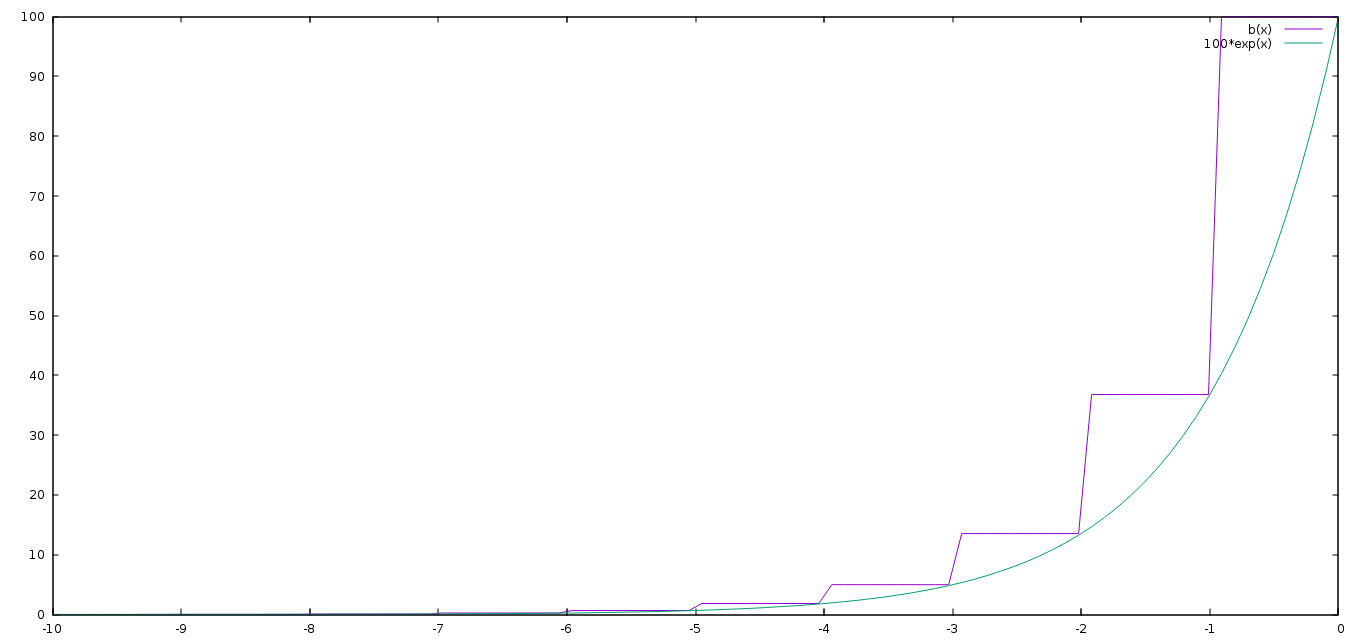
\includegraphics [width=5in]{images/a_u_b.eps}
        \caption{$Me^{-t}$ e $B(t)$ descrescono alla stessa velocità per $\alpha = e$}
    \end{center}
\end{figure}

In figura si mostra la validità della dimostrazione, avendo posto $\alpha = e$. In tal caso le funzioni decrescono alla stessa velocità (infatti per ogni valore di $x$ discreto, le due funzioni assumono lo stesso valore).

\clearpage
\section{NERDZ}
\begin{wrapfigure}{r}{0.25\textwidth}
    \setlength\intextsep{0pt}
    \begin{center}
        \raisebox{0pt}[\dimexpr\height-2\baselineskip\relax]{
\includegraphics[width=0.2\textwidth]{images/N.png}}
        \caption{Logo di NERDZ.}
        \vspace*{-1cm}
    \end{center}
\end{wrapfigure}
NERDZ è una piattaforma di social networking, cioè è un insieme di\\ sistemi software interagenti creati per costruire social network (reti sociali) e per favorire la costruzione di relazioni sociali tra persone che condividono gli stessi interessi, svolgono le stesse attività o sono collegati tra di loro nella vita reale.

La nascita di questa piattaforma risale al 2010, anno in cui decisi di creare un luogo di incontro e crescita per le persone che condividevano i miei stessi interessi, cioè persone appartenenti alla \textbf{Cyberculture}.

\begin{quotation}
    \noindent{La Cyberculture o computer culture è la cultura che è emersa, o sta emergendo, dall'uso delle reti di computer come mezzi di comunicazione, divertimento e lavoro.

    È intesa anche come lo studio di diversi fenomeni sociali associati ad internet ed altre nuove forme di comunicazione in rete (online community, online multiplayer games, wearable computing, social gaming, i social media, realtà aumentata, ecc...) ed include questioni relative all'identità, alla privacy ed alla formazioni della reti.}\textsuperscript{\cite{wiki_cyberculture}}
\end{quotation}

In particolare, NERDZ venne creato per dare una nuova forma ai forum che trattavano di informatica e argomenti correlati.

I forum (o message board) sono luoghi di discussione online in cui gli utenti intrattengono conversazioni mediante l'azione di invio di messaggi sotto forma di post.

In quel periodo ci fu l'esplosione dei più popolari social network (in particolare di Facebook \footnote{http://www.facebook.com/}) ed i forum si spopolarono rapidamente a favore del popolamento di semplici pagine dei social network nelle quali, però, la qualità delle informazioni scambiate era molto bassa e ognuno per poter partecipare era obbligato ad avere un account del social network, account che richiede l'immissione di informazioni personali reali e verificabili.

Data la perdita totale di anonimato che i classici social network comportano, decisi di realizzare NERDZ facendo in modo che venissero preservate le caratteristiche peculiari dei forum, delle quali l'anonimato era una di particolare rilievo.
\clearpage
\begin{thebibliography}{9}
    \bibitem{wiki_cyberculture}
        \emph{Cyberculture - Wikipedia}.
        http://en.wikipedia.org/wiki/Cyberculture

    \bibitem{wiki_hashtag}
        \emph{Hashtag - Wikipedia}
        http://it.wikipedia.org/wiki/Hashtag

    \bibitem{ref0}
        \emph{Recommender Systems Wiki (RecSysWiki)}
        http://recsyswiki.com/wiki/Main\_Page

    \bibitem{contentwise_tv}
        \emph{Do Metrics Make Recommender Algorithms?}
        http://www.contentwise.tv/files/Do-Metrics-Make-Recommender-Algorithms.pdf

    \bibitem{ref1}
        \emph{Sensivity and Specificity}
        https://en.wikipedia.org/wiki/Sensitivity\_and\_specificity

    \bibitem{ref2}
        \emph{Precision and Recall}
        https://en.wikipedia.org/wiki/Precision\_and\_recall

\end{thebibliography}

\end{document}
